\chapter{Market data: from the SPX chain to forwards and discount factors}
\chaptermark{Market data}
\label{cap:dati}

For each expiry, every model needs three numbers: the forward $F$, the discount factor $\DF$ and the time $T$. In
addition, the calibration (Chapter~\ref{cap:calibrazione}) needs a ``clean'' price surface.

This chapter explains how the project obtains all of this from a single \emph{snapshot} of the S\&P\,500 option
quotes, \emph{without assuming} any rate curve or dividend yield. The processing pipeline has six stages:
\begin{enumerate}
\item the raw snapshot, saved once and for all;
\item the choice of a single contract family per date and the computation of the time to expiry;
\item the quote-cleaning filters;
\item the put--call parity regression, which gives $F$ and $\DF$ for each expiry;
\item the correction of the short-dated discount factors with a smooth rate curve, and the recomputation of the
forwards;
\item the OTM surface, cleaned of static arbitrage, which is the input to the calibration.
\end{enumerate}

\section{What an option chain contains}
An \textbf{option chain} is the list of all the options quoted on an underlying. For each expiry and each strike it
contains calls and puts with:
\begin{itemize}
\item the \emph{bid} price, at which someone is willing to buy;
\item the \emph{ask} price, at which someone is willing to sell;
\item the \emph{open interest} (number of open contracts) and the date of the last trade.
\end{itemize}
The reference price is the \emph{mid} $=(\text{bid}+\text{ask})/2$. The half-spread $(\text{ask}-\text{bid})/2$
measures the uncertainty of the quote: any ``true'' price inside the bid/ask band is consistent with the market.

\begin{progetto}
The snapshot was downloaded from Yahoo Finance (\code{scripts/fetch\_spx.py}) on \mbox{2026-11-06} at 22:13:53 UTC,
after the US close: 15{,}843 rows, 40 expiries from 7 days to 2 years. The raw file is saved together with the spot
and the timestamp; everything else is recomputed by scripts (\code{scripts/build\_market.py}), and the intermediate
tables go to \code{data/processed/}.
\end{progetto}

\section{Two details that look like red tape and are not}
\subsection{AM and PM options}
Two families coexist in the Yahoo chain:
\begin{itemize}
\item \texttt{SPX}: standard monthlies and LEAPS, settled in the morning (\textbf{AM}) on the special opening quotation
(SOQ);
\item \texttt{SPXW}: weeklies, end-of-month and quarterlies, settled in the afternoon (\textbf{PM}) on the closing
price.
\end{itemize}
The same Friday can have both. But they are different contracts: they settle on different prices and at different
times (6.5 hours apart, about ${7.4\times10^{-4}}$ years). Mixing them in the same regression or in the same smile is
wrong.

The project keeps \emph{a single family per date} and prefers SPX, which is much more liquid on those dates: for
example, 139 against 44 clean call/put pairs. Keeping only SPXW, conversely, would have removed the 11 long expiries
that exist only as SPX, and with them the 2-year surface. On the five dates where the two families overlap, the
forwards agree within 0.27 index points: the choice does not move $F$.

\subsection{Time to expiry}
Time is measured in calendar years, with the ACT/365F convention:
\begin{equation}\label{eq:tempo-act365}
T=\frac{\text{seconds between the snapshot and the settlement instant}}{365\cdot86{,}400}.
\end{equation}
The settlement instant is 09:30 New York time for AM options and 16:00 for PM options. On early-close days, however,
the close (and therefore the PM settlement) is at 13:00.

This detail emerged from an independent check. For example, for the SPXW expiry of \mbox{2026-11-27} (the day after
Thanksgiving) the time goes from 0.0573937 to 0.0570512 years: three hours less. On the very short expiries a few
hours visibly change the implied rate, which on that expiry went from 5.643\% to 5.677\%. The early-close days for
2026--2028 are listed in \code{data.EARLY\_CLOSE}.

\section{Cleaning the quotes}
After the close Yahoo might show zero bids and asks; in the snapshot they are instead populated (only 471 rows out
of 14{,}707, 3.2\%, have a zero or missing bid). The filters are applied in the order of Table~\ref{tab:filtri}, and
every step is counted.

\begin{table}[htbp]
\centering
\small
\caption{Cleaning filters for the snapshot, in the order in which they are applied.}
\label{tab:filtri}
\begin{tabular}{@{}lr@{}}
\toprule
step & rows left\\
\midrule
raw & 15{,}843\\
one family per date & 14{,}707\\
bid $>0$ & 14{,}236\\
ask finite and $\ge$ bid & 14{,}228\\
(ask $-$ bid)/mid $\le0.5$ & 13{,}608\\
open interest $>0$ & 12{,}956\\
OTM cut (39 expiries) & 7650\\
static-arbitrage filter & 7625\\
\bottomrule
\end{tabular}
\end{table}

A missing value never passes a filter, and it is counted: no row disappears without a trace. The contract symbols
are also checked against the strike, type and expiry columns; a mismatch stops the program. The last two steps are
explained later (Sections~\ref{sec:superficie-otm} and~\ref{sec:filtro-arbitraggio}).

\section{Forward and discount factor from put--call parity}
\subsection{The idea}
Parity (Proposition~\ref{prop:parita}) says that, for every strike $K$ of a given expiry,
\begin{equation}\label{eq:parita-regressione}
y(K):=C(K)-P(K)=\DF\cdot F-\DF\cdot K .
\end{equation}
As a function of $K$ this is a \textbf{straight line} with intercept $a=\DF\cdot F$ and slope $b=-\DF$. If I measure
$C-P$ over many strikes and run a linear regression on $K$, I read off
\begin{equation}\label{eq:F-DF-da-retta}
\DF=-b,\qquad F=\frac{a}{\DF}=\bar K-\frac{\bar y}{b},\qquad r=-\frac{\ln\DF}{T}.
\end{equation}
No rate, no dividend, no spot, no model: only European option prices. Geometrically, $F$ is the point where the line
crosses zero (there call and put are worth the same), and $\DF$ is its slope with the sign flipped.

\begin{perche}[title={Why not simply use spot, rate and dividend?}]
\begin{itemize}
\item The index dividends are discrete and uncertain, and the stock-borrow cost is not observable. An assumed $q$
gets $F$ wrong, so it shifts all the moneyness values $k=\ln(K/F)$ and makes the implied volatilities of calls and
puts at the same strike diverge (a spurious skew).
\item The Yahoo spot is not synchronous with the options: the 7-day forward comes out 0.13\% above the spot 7376.86,
which would imply an annual carry of about 6.7\%, a meaningless value. The spot is therefore kept only for
information and does not enter any computation.
\item The forward extracted from parity is \emph{by construction} consistent with the option prices, and the quality
of the fit is also a check on the quality of the data.
\end{itemize}
What $F$ contains: $F=(S_0-\mathrm{PV}(\text{div}))/\DF$, that is, the \emph{net} carry (rates minus dividends minus
stock borrow). Parity returns the implied dividend, not a separate dividend curve.
\end{perche}

\subsection{A refresher: linear regression (OLS) and its errors}
Given $n$ points $(K_i,y_i)$, ordinary least squares chooses the $a,b$ that minimize $\sum_i(y_i-a-bK_i)^2$. Denote by
$\bar K,\bar y$ the means, by $K_i^c=K_i-\bar K$ the centered strikes and by $S_{xx}=\sum_i(K^c_i)^2$. The solutions
are
\begin{equation}\label{eq:ols}
b=\frac{\sum_iK^c_i(y_i-\bar y)}{S_{xx}},\qquad a=\bar y-b\bar K,\qquad
s^2=\frac{\sum_i\text{res}_i^2}{n-2},\qquad \SE(b)=\frac{s}{\sqrt{S_{xx}}}.
\end{equation}
The coefficient $R^2=1-\sum\text{res}^2/\sum(y-\bar y)^2$ measures the fraction of the variability explained by the
line.

\paragraph{The standard error of \texorpdfstring{$F$}{F}, step by step.} $F=\bar K-\bar y/b$ is a nonlinear function
of two estimators, $\bar y$ and $b$. One uses the \emph{delta method}: linearize $F$ around the estimated values and
propagate the variance.
\begin{enumerate}
\item \emph{The two sources of error.} $\bar y$ has variance $s^2/n$ (the mean of $n$ residuals of variance $s^2$);
$b$ has variance $s^2/S_{xx}$. With centered strikes, $\bar y$ and $b$ are \emph{uncorrelated}.
\item \emph{The derivatives.} $\partial F/\partial\bar y=-1/b$ and $\partial F/\partial b=\bar y/b^2$.
\item \emph{The sum of the variances.} Since the two estimators are uncorrelated, the variances add with no cross
term:
\begin{equation}\label{eq:se-F}
\SE(F)^2=\frac{1}{b^2}\cdot\frac{s^2}{n}+\frac{\bar y^2}{b^4}\cdot\frac{s^2}{S_{xx}}
=\frac{s^2}{n\,b^2}+\frac{\bar y^2\,s^2}{S_{xx}\,b^4}.
\end{equation}
\end{enumerate}
The code is \code{market.ols\_parity}. The implied rate is $r=-\ln\DF/T$, and its standard error is
$\SE(r)=\SE(b)/(\DF\,T)$.

\begin{attenzione}[title={Why center the strikes}]
SPX strikes are around 7400: the normal equations with raw $K$ are ill-conditioned (huge, nearly equal numbers are
subtracted). Working with $K-\bar K$ removes the problem, and in addition intercept and slope become uncorrelated
estimators, which is exactly what allowed us to write \eqref{eq:se-F} with no cross term.
\end{attenzione}

\section{Robust regression and stale quotes}
\subsection{The window near the forward}
A \emph{pair} is a strike with both a clean call and a clean put. Not all pairs are used, only the 20 closest to the
forward (at least 10 valid pairs are required): deep ITM legs have wide spreads and often \emph{stale} prices.

A first, approximate forward is taken where $C-P$ changes sign: at the strike $K^*$ with the smallest $|C-P|$ one sets
$F_0=K^*+(C-P)(K^*)$, which is \eqref{eq:parita-regressione} solved with $\DF\approx1$.

\subsection{Theil--Sen and MAD}
Some prices are simply wrong, because they have not been updated. A real example, on the \mbox{2027-03-31} expiry:
the 7455 put was quoted 212.9/214.9, while the 7450 and 7460 puts were quoted 317.8/319.3 and 321.3/322.9. The 7455
was stuck at a price from months earlier.

Least squares is very sensitive to such outliers: on three expiries OLS on the 20-pair window gave $R^2$ equal to
0.12, 0.39 and 0.93. The project uses two robust tools:
\begin{itemize}
\item \textbf{Theil--Sen}: the slope is the \emph{median} of the slopes between all pairs of points, and the
intercept is the median of $y_i-bK_i$. It tolerates up to $1-1/\sqrt2\approx29.3\%$ of outliers (its
\emph{breakdown point}).
\item \textbf{MAD}: the median absolute deviation of the residuals; $1.4826\cdot\mathrm{MAD}$ estimates the standard
deviation as $s$ would for Gaussian data, but without being influenced by the outliers.
\end{itemize}

\subsection{The ``inside the band'' rejection rule}
Each pair has its own quote uncertainty. The synthetic forward $C-P$ is bought at $C^a-P^b$ and sold at $C^b-P^a$,
so its half-spread is
\begin{equation}\label{eq:semiampiezza-cp}
h_i=\tfrac12\big[(C^a_i-P^b_i)-(C^b_i-P^a_i)\big]=\tfrac12(C^a_i-C^b_i)+\tfrac12(P^a_i-P^b_i).
\end{equation}
With $e_i$ the residual from the Theil--Sen line, pair $i$ is rejected if and only if
\begin{equation}\label{eq:regola-scarto}
|e_i|>\max\big(4\cdot1.4826\cdot\mathrm{MAD}(e),\;h_i\big).
\end{equation}
In words: a pair is excluded only if its residual exceeds 4 robust deviations \emph{and} the robust line falls
outside its bid/ask band. A pair whose band contains the line is never rejected, even if its residual is large
compared with the others.

Then OLS \eqref{eq:ols} is rerun on the remaining pairs. Both legs of a rejected strike are also removed from the
surface, because parity cannot tell which of the two is stale.

\begin{progetto}
The rule rejects 9 strikes in 3 expiries (4 + 4 + 1); on the other 36 retained expiries no pair is rejected. The three
expiries that had $R^2$ equal to 0.12, 0.39 and 0.93 with plain OLS reach about 0.99998.
\end{progetto}

\subsection{When an expiry is accepted}
An expiry is kept only if \emph{all} these conditions hold:
\begin{enumerate}
\item at least 10 pairs, before and after rejection;
\item rejected fraction $<0.293$ (below the Theil--Sen breakdown point);
\item $R^2>0.999$;
\item the final line passes inside the band of \emph{every} pair used: $\max_i|\text{res}_i|/h_i\le1$;
\item $\DF\in(0.8,1]$.
\end{enumerate}
Otherwise it is discarded, and the reason is recorded.

The function \code{market.implied\_forwards} applies these rules to all expiries.

\begin{perche}[title={Why is $R^2>0.999$ not enough?}]
\begin{enumerate}
\item $R^2$ grows with the width of the strike interval: it is not a uniform criterion across expiries. With strikes
spaced 5 points apart and 10 pairs, $R^2>0.999$ requires a root-mean-square residual below about 0.45 index points,
a threshold that changes with the window.
\item With 20 points the MAD is itself noisy, and rejecting points can ``rescue'' a chain of pure noise. An
independent check on synthetic pure-noise chains (noise of 2 points, half-spread 0.5) showed that, with the
rejection rule alone, 4 chains out of 500 passed $R^2>0.999$. With conditions 2 and 4 this drops to 0 out of 500.
\item ``The line passes inside the band of every quote'' has a clear economic content: the fit is consistent with
tradable prices.
\end{enumerate}
Iteratively rejecting the worst point until $R^2$ passes is, by contrast, forbidden: it is exactly how one ``eats''
the noise until the test is passed.
\end{perche}

\begin{attenzione}[title={The price of the ``inside the band'' rule}]
Condition 4 looks at the \emph{single} worst pair, so it can eliminate a valid but noisy expiry because of one
marginal quote. On valid synthetic chains (exact parity plus Gaussian noise) the fraction of expiries kept is 100\%,
99.9\%, 96.5\% and 55.6\% with noise equal to 0.2, 0.3, 0.35 and 0.5 times the half-spread. On the real snapshot the
ratio of noise to half-spread ranges from 0.044 to 0.372. The rule is conservative: an expiry can be lost, but a
wrong forward is never accepted. This is a deliberate choice.
\end{attenzione}

\begin{progetto}
Result: 39 expiries out of 40 kept. Only \mbox{2026-12-08} is discarded, which has 7 clean pairs out of the 10
required.
\begin{itemize}
\item Minimum $R^2$ 0.999941 (\mbox{2027-02-19}); $\DF\in[0.923895,\,0.998395]$; standard error of $F$ between 0.03
and 0.40 points.
\item Margin on the rules: $\max|\text{res}|/h=0.814$ against 1 (\mbox{2026-11-18}); maximum rejected fraction
$4/20=0.20$ against 0.293.
\item A second, independent method (L1 regression, with no rejection at all) agrees within 3 standard errors: at
most 1.87~SE on $F$ and 2.43~SE on $\DF$.
\item With windows of 10, 20 and 40 pairs, 34, 39 and 38 expiries are kept, and $F$ changes by at most
${2.09\times10^{-4}}$ in relative terms.
\end{itemize}
A single expiry, \mbox{2026-12-07}, has its forward outside the range of the strikes used (13 pairs with
$K\in[7425,7800]$, $F=7396.42$): it is kept with a warning, and its extrapolation shows up in the larger standard
error, 0.40 points.
\end{progetto}

\section{Why \texorpdfstring{$F$}{F} is well determined and (short-dated) \texorpdfstring{$\DF$}{DF} is not}
Look at \eqref{eq:se-F}: the second term, the only one containing the slope uncertainty, is multiplied by
$\bar y^2$. If the strike window is centered around the forward, $\bar y=\DF(F-\bar K)\approx0$ and \emph{the slope
uncertainty does not propagate to $F$}. $F$ is the point where the line crosses zero, and that point is robust.

The slope, on the other hand, is $-\DF$, and what distinguishes it from $-1$ is $1-\DF$. On a window of width
$\Delta K$, the useful signal is $(1-\DF)\Delta K$. For an expiry of one or two weeks this is about 0.05--0.1 index
points, that is, \emph{less than the resolution of the quotes}. The fit does not ``see'' the slope: it sees noise and
small asymmetries of the ITM quotes. The zero crossing, instead, remains much better determined: the standard error
of $F$ lies between 0.03 and 0.40 points on all expiries, even the shortest.

\begin{progetto}[title={In the qpricer project: the raw implied rates}]
\begin{itemize}
\item For $T<0.1$ the implied rates swing between 2.64\% and 16.89\% (standard error 0.4\%--4.3\%).
\item For $T>0.3$ they lie between 4.5\% and 5.1\% (standard error $\le0.36\%$).
\item The discount factor \emph{increases} with $T$, which is impossible with positive rates, 10 times out of 38
between consecutive expiries.
\item Going from 20 to 40 pairs moves the short-dated $\DF$s by up to 9.9 standard errors: the standard error
computed from the residuals underestimates the true uncertainty.
\end{itemize}
Widening the window raises the short rates: this is the sign of a systematic distortion of the ITM quotes, not of
pure noise. $F$, by contrast, is unaffected (standard error $\le0.4$ points).
\end{progetto}

\begin{idea}[title={What rate is the parity rate?}]
The difference between the parities at two strikes is $[C-P](K_1)-[C-P](K_2)=\DF\,(K_2-K_1)$: the price of a
\emph{box spread}, that is, a riskless loan of $K_2-K_1$. The parity rate is therefore the rate implied by box spreads
(a funding rate), not the risk-free OIS rate. The 4.5\%--5.1\% of the long expiries should be read this way; the
16.9\% over two weeks is not a rate, it is noise.
\end{idea}

\section[Correcting the short end: rate curve and recomputed forward]{Correcting the short end:\\
rate curve and recomputed forward}
\label{sec:breve-termine}
The short-dated discount factors are not identified. Before inverting prices into implied volatilities for the
calibration, the project replaces them with a smooth curve estimated on the long end, where the $\DF$s are reliable,
and then recomputes the forwards at fixed $\DF$. The code is \code{calibration.\allowbreak smooth\_short\_end}.

\subsection{How much an error on \texorpdfstring{$\DF$}{DF} or on \texorpdfstring{$F$}{F} matters}
Before correcting, it pays to understand what is being corrected.

\textbf{Step 1: what the inversion sees.} The implied volatility of an OTM option depends only on the undiscounted
price $v=V/\DF$ and on $F$ (Chapter~\ref{cap:black}). An error on $\DF$ rescales $v$: $\delta v/v=-\delta\DF/\DF$.

\textbf{Step 2: from price to volatility.} To first order $\delta\sigma=\delta v/\vega_u$, where
$\vega_u=\partial v/\partial\sigma=F\varphi(d_1)\sqrt T$ is the undiscounted vega. Hence
\begin{equation}\label{eq:dsigma-dDF}
\delta\sigma=-\frac{v}{\vega_u}\,\frac{\delta\DF}{\DF}=-\sigma\,E\,\frac{\delta\DF}{\DF},
\qquad E:=\frac{v}{\sigma\,\vega_u}.
\end{equation}
$E$ is the inverse of the elasticity of the price with respect to volatility. At the money $E=1+s^2/12+O(s^4)$, with
$s=\sigma\sqrt T$; in the wings it becomes small ($E\approx1/(|d_1||d_2|)$). The worst case is therefore at the
money, where a relative error on $\DF$ becomes the same relative error on $\sigma$.

\textbf{Step 3: an error on $F$ at fixed price.} If $v$ stays the same and $F$ changes, then
$0=\delta v=\theta\Phi(\theta d_1)\,\delta F+\vega_u\,\delta\sigma$, so
\begin{equation}\label{eq:dsigma-dF}
\delta\sigma=-\frac{\theta\,\Phi(\theta d_1)}{\varphi(d_1)\sqrt T}\cdot\frac{\delta F}{F}
\;\overset{\text{ATM}}{\approx}\;\mp1.2533\,\frac{\delta F}{F\sqrt T},
\end{equation}
because at the money $\Phi(d_1)\approx\tfrac12$ and $\varphi(0)=1/\sqrt{2\pi}$, and $\tfrac12\sqrt{2\pi}=1.2533$. The
sign depends on $\theta$: an overestimated forward ($\delta F>0$) lowers the volatility of the calls and raises that
of the puts. In other words, it creates a \emph{gap} between the call and put volatilities at the same strike, which
the model would then mistake for skew.

\begin{esempio}[title={Example: the worst expiry (estimate)}]
The most distorted parity $\DF$ is that of \mbox{2026-11-19}: $T=0.0355$, $r=16.89\%$, $\DF=0.994027$. The smooth curve
gives $\widetilde{\DF}=0.998391$. The relative error is about $0.43\%$, so by \eqref{eq:dsigma-dDF} the ATM
volatility is shifted by about $0.43\%$ of $\sigma$: $0.065$ vol points at $\sigma=15\%$. This is small, but it is
\emph{systematic}: it moves the whole smile of that expiry in the same direction.
\end{esempio}

\subsection{The zero-rate curve}
A straight line is fitted for the zero rate as a function of expiry,
\begin{equation}\label{eq:curva-zero}
\hat r(T)=a+b\,T,
\end{equation}
by \textbf{weighted least squares} (WLS) on the 21 expiries with $T\ge0.1$, where parity identifies $\DF$ well. One
minimizes
\begin{equation}\label{eq:wls}
\sum_{j:\,T_j\ge0.1}w_j\big(r_j-a-bT_j\big)^2,\qquad w_j=\frac{1}{r_{\mathrm{se},j}^2+s_0^2},\qquad s_0=10\text{ bp}.
\end{equation}
The weight gives more importance to the expiries with a more precise rate. The \emph{floor} $s_0$ is needed because
the standard error $r_{\mathrm{se}}$ computed from the residuals underestimates the true uncertainty (we have seen it:
the choice of window alone moves the $\DF$s well beyond their standard errors). Without a floor, an expiry with an
accidentally small $r_{\mathrm{se}}$ would dominate the curve.

Then:
\begin{equation}\label{eq:DF-curva}
\widetilde{\DF}_j=
\begin{cases}
\exp\big(-\hat r(T_j)\,T_j\big) & \text{if } T_j<0.1 \quad\text{(18 expiries)},\\
\DF_j\ \text{(parity)} & \text{if } T_j\ge0.1 .
\end{cases}
\end{equation}

\begin{perche}[title={Why a straight line, and why not an external OIS curve?}]
\begin{itemize}
\item An external (OIS) curve would break the principle of Chapter~\ref{cap:opzioni}: all the carry comes from the
options themselves, and the parity rate is a funding rate, not OIS.
\item The shape of the curve matters little. Any $\hat r$ within $\pm0.5\%$ of the true value moves the volatilities
at $T<0.1$ by at most 0.01 vol points (estimate from \eqref{eq:dsigma-dDF}: $\delta\DF/\DF=\delta r\cdot
T\le0.005\cdot0.1$).
\item Using the curve on \emph{all} expiries would not help: where parity identifies $\DF$, the direct data are
better than a model.
\end{itemize}
\end{perche}

\subsection{The forward at fixed \texorpdfstring{$\DF$}{DF}}
Changing $\DF$ also changes $F$, because the parity line must still pass through the data. With $\widetilde{\DF}$
fixed, \eqref{eq:parita-regressione} has a single unknown.

\textbf{Step 1: the one-parameter fit.} On the same pairs used before ($n_u$ pairs, means $\bar K_u$ and $\bar y_u$)
one minimizes $\sum_i\big(y_i-\widetilde{\DF}(F-K_i)\big)^2$ over $F$. Setting the derivative to zero:
\[
\sum_i\big(y_i-\widetilde{\DF}\,F+\widetilde{\DF}\,K_i\big)=0
\quad\Longrightarrow\quad
\tilde F=\bar K_u+\frac{\bar y_u}{\widetilde{\DF}},\qquad
\SE(\tilde F)=\frac{s_u}{\widetilde{\DF}\sqrt{n_u}},
\]
with $s_u$ the standard deviation of the residuals.

\textbf{Step 2: comparison with the parity forward.} The OLS line also passes through the centroid
$(\bar K_u,\bar y_u)$, with $\bar y_u=\DF(F-\bar K_u)$, so $F=\bar K_u+\bar y_u/\DF$. Subtracting:
\begin{equation}\label{eq:spostamento-F}
\tilde F-F=\bar y_u\Big(\frac1{\widetilde{\DF}}-\frac1{\DF}\Big)
=\frac{(F-\bar K_u)\,(\DF-\widetilde{\DF})}{\widetilde{\DF}} .
\end{equation}

\textbf{Step 3: interpretation.} The shift is the product of two small quantities: the distance between the center
of the window and the forward, and the correction to $\DF$ (of order $10^{-3}$). This is the same reason why $F$ was
well determined even when $\DF$ was not. For $T\ge0.1$ we have $\widetilde{\DF}=\DF$, and \eqref{eq:spostamento-F}
returns exactly the parity forward.

\textbf{Step 4: redo the OTM cut.} A strike falling between $F$ and $\tilde F$ would change type (from OTM put to
OTM call or vice versa). For this reason the OTM cut and the static-arbitrage filter are redone with $\tilde F$
(\code{calibration.\allowbreak recut\_surface}).

\subsection{Results on the snapshot}

\begin{progetto}[title={In the qpricer project: the short-end correction}]
\begin{itemize}
\item Fitted curve: $\hat r(T)=4.527\%+0.304\%\cdot T$.
\item The short rates go from 2.64\%--16.89\% to 4.533\%--4.556\%. The sequence of $\DF$s below $0.1$ years becomes
monotonic.
\item The number of $\DF$s that increase between consecutive expiries goes from 10 to 4. Three of these lie at
$T\ge0.1$, where the parity $\DF$s are kept by choice; the fourth is the step across $T=0.1$, from the curve $\DF$
0.99565 (\mbox{2026-12-11}) to the parity $\DF$ 0.99609 (\mbox{2026-12-18}).
\item Forwards: the largest shift is $|\tilde F-F|=3.56$ standard errors (\mbox{2026-12-03}, $+0.654$ points). Four
short expiries exceed 2 standard errors (2.21, 2.37, 2.82 and 3.56): more than estimated a priori (about 1.5),
because there the parity $\DF$s were too low by up to 0.4\%.
\item Every pair used stays inside its own bid/ask band also with $(\tilde F,\widetilde{\DF})$:
$\max|\text{res}|/h=0.834$, no pair above 1.
\item On the 347 strikes used with $T<0.1$, the median gap between the call and put volatilities at the same strike
falls from 0.0275 to 0.0260 vol points; the pairs whose gap exceeds the sum of the two half-spreads in volatility
remain 0.
\item The recut surface is identical to the original one: 7625 quotes, no strike changes type, because no quoted
strike falls between $F$ and $\tilde F$.
\end{itemize}
The automated checks (\code{scripts/phase5\_gates.py}) also verify that the correction leaves $F$ and $\DF$ unchanged
for $T\ge0.1$ (measured difference exactly 0), that WLS exactly recovers a known linear curve
(${6.9\times10^{-18}}$) and that the market implied volatilities, fed back into Black's formula, reproduce the 7625
prices with a maximum relative error of ${3.9\times10^{-13}}$.
\end{progetto}

Table~\ref{tab:breve-termine} shows a few expiries; Figure~\ref{fig:df-r} shows the whole term structure before and
after the correction. The file \code{report/calibration\_f5\_20261106\_2213.csv} reports the values for all expiries.

\begin{table}[htbp]
\centering
\small
\caption{Short-end correction on a few expiries. $r$: parity rate; $\tilde r$: rate after \eqref{eq:DF-curva};
$z_F=(\tilde F-F)/\SE(F)$; the last column is $\max|\text{res}|/h$ with $(\tilde F,\widetilde{\DF})$.}
\label{tab:breve-termine}
\begin{tabular}{@{}lrrrrrr@{}}
\toprule
expiry & $T$ & $r$ & $\tilde r$ & $\tilde F-F$ (points) & $z_F$ & $\max|\text{res}|/h$\\
\midrule
\mbox{2026-11-13} & 0.0190 & 8.44\% & 4.533\% & 0.01 & 0.30 & 0.491\\
\mbox{2026-11-18} & 0.0327 & 16.33\% & 4.537\% & 0.36 & 2.21 & 0.834\\
\mbox{2026-11-19} & 0.0355 & 16.89\% & 4.538\% & 0.46 & 2.37 & 0.582\\
\mbox{2026-12-03} & 0.0738 & 9.19\% & 4.550\% & 0.65 & 3.56 & 0.495\\
\mbox{2026-12-07} & 0.0848 & 8.33\% & 4.553\% & 0.79 & 1.96 & 0.437\\
\mbox{2026-12-18} & 0.1142 & 3.44\% & 3.44\% & 0 & 0 & 0.194\\
\bottomrule
\end{tabular}
\end{table}

\begin{figure}[htbp]
\centering
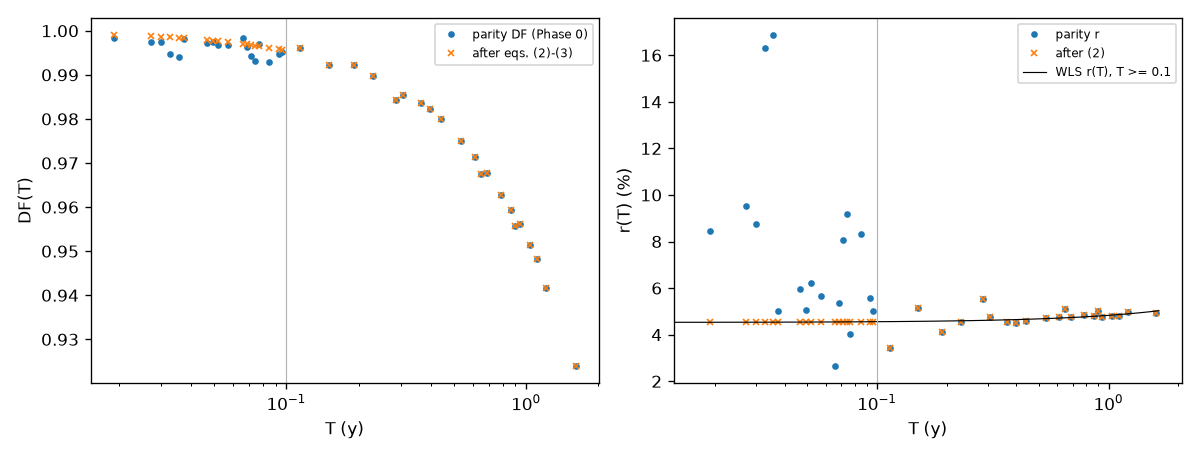
\includegraphics[width=\textwidth]{calibration_df_r_20261106_2213.png}
\caption{Term structure of the discount factors (left) and of the zero rates (right), on a logarithmic scale in $T$.
Dots: parity values; crosses: after the short-end correction; line: the WLS curve fitted for $T\ge0.1$ (vertical
line). Below $0.1$ years the parity rates swing between 2.6\% and 16.9\%; after the correction they lie on the
curve.}
\label{fig:df-r}
\end{figure}

\begin{idea}
The correction changes almost nothing in the calibration numbers (the call/put gap barely decreases), but it removes
meaningless rates and a systematic error on the whole smile of the weekly expiries. It is the kind of correction that
is made \emph{before} inverting the prices, because afterwards the error would be hidden inside the model
parameters.
\end{idea}

\section{The OTM surface}
\label{sec:superficie-otm}
For the calibration only \textbf{out-of-the-money} options are kept: puts for $K<F$, calls for $K\ge F$
(\code{data.select\_otm}).

\begin{perche}
The price of an ITM option is almost all intrinsic value. The bid/ask spread, which is in absolute terms, falls
entirely on the small time value and becomes a large error on the implied volatility (Chapter~\ref{cap:black}). OTM
options are more liquid and have tighter relative spreads.

And no information is lost: if $F$ and $\DF$ are consistent with parity, the call and the put at the same strike have
the same implied volatility.
\end{perche}

\section{The static-arbitrage filter}
\label{sec:filtro-arbitraggio}
Even after cleaning, some stale quotes remain that create obvious arbitrages. The parity rejection rule only sees the
20-pair window; the wings of the surface and the strikes without a twin leg escape it.

For two strikes $K_i<K_j$ of the same expiry and of call type, using \emph{tradable} prices (bid and ask, not the
mid):
\begin{itemize}
\item \emph{monotonicity:} if $\text{bid}_j>\text{ask}_i$, I buy the low-strike call and sell the high-strike one,
collecting a credit, with a future payoff $\ge0$: an arbitrage;
\item \emph{vertical spread:} if $\text{bid}_i-\text{ask}_j>K_j-K_i$, I sell a spread for more than its maximum
payoff.
\end{itemize}
For puts the conditions are mirrored: $\text{bid}_i>\text{ask}_j$ or $\text{bid}_j-\text{ask}_i>K_j-K_i$. Using
$\DF\le1$ makes the conditions independent of any model.

All pairs of strikes are checked, not only adjacent ones, because a stale quote can violate monotonicity with a
distant strike.

The function \code{data.remove\_static\_arbitrage} ``greedily'' removes the quote involved in the largest number of
violations (ties broken by the least recently traded, then by the lowest strike) and repeats until none are left. A
stale quote conflicts with every good quote it crosses, so it has far more violations than the others.

\begin{esempio}
On the \mbox{2027-03-31} expiry the 7615 call had a bid of 434.4 while the 7610 call was offered at 258.5: buying the
7610 and selling the 7615 would have yielded a credit of 175.9 points with a payoff that is never negative. Its
implied volatility was 26.7\%, against about 17\% for its neighbors.

In total 25 quotes were removed on 5 expiries. They were all stale (last trade between July and September 2026) and
14.4--179.9 points away from the level indicated by their neighbors. An independent check, with a different
algorithm, confirmed that the resulting surface has no violations and that each of the 25 removals is necessary:
putting any one of them back makes the arbitrage reappear.
\end{esempio}

\begin{attenzione}
The filter guarantees only monotonicity and vertical spreads. Convexity (butterfly) and calendar arbitrage are
checked, as diagnostics, in the calibration (Chapter~\ref{cap:calibrazione}). On the final surface there are no
violations executable at bid/ask, neither calendar (11{,}054 points) nor butterfly (7547 triples). On the mids,
however, 2126 triples violate convexity, all by less than half the spread of the butterfly (at most 0.427 times): the
mid is not a tradable price. Saying ``the surface is arbitrage-free'' without these qualifications would be wrong.
\end{attenzione}

\begin{riassunto}
\begin{itemize}
\item One family per date (AM/PM), ACT/365F time to the settlement instant (watch out for early closes).
\item $C-P=\DF F-\DF K$: a straight line in $K$; slope $=-\DF$, zero $=F$. $F$ is robust (because $\bar y\approx0$),
short-dated $\DF$ is not.
\item Robust regression (Theil--Sen, MAD) and rejection only outside the bid/ask band; the acceptance rules have an
economic content and do not stop at $R^2$. 39 expiries out of 40 remain.
\item At the short end the $\DF$s are replaced by a curve $\hat r(T)=4.527\%+0.304\%\,T$ fitted on $T\ge0.1$, and the
forwards are recomputed at fixed $\DF$: shifts below one index point, pairs always inside their bands.
\item OTM surface, static-arbitrage filter on bid/ask: 7625 quotes on 39 expiries.
\end{itemize}
\end{riassunto}

\begin{domande}
\begin{enumerate}
\item How do you obtain $F$ and $\DF$ from an option chain without knowing $r$ and $q$?
\item Why is the forward identified even at very short expiries while the discount factor is not? \emph{Hint:}
\eqref{eq:se-F} with $\bar y\approx0$.
\item Is the 16.9\% rate on a two-week expiry real? \emph{Hint:} no, the slope signal is below the resolution of the
quotes; the long rate is the box-spread rate.
\item Why does the rejection rule require the line to be outside the bid/ask band?
\item Derive the shift \eqref{eq:spostamento-F} of the forward when $\DF$ is changed. Why is it small?
\item How much does a 0.4\% error on $\DF$ move the ATM volatility? And an error on $F$? \emph{Hint:}
\eqref{eq:dsigma-dDF} and \eqref{eq:dsigma-dF}.
\item Why are bid and ask, and not the mid, used in the arbitrage filter? \emph{Hint:} only an arbitrage executable at
the quoted prices is a true arbitrage.
\end{enumerate}
\end{domande}
